\documentclass{boi2014-de}

\usepackage{enumitem}
\usepackage{todonotes}
\usepackage{wrapfig}

\renewcommand{\DayNum}{2}
\renewcommand{\TaskCode}{demarcation}
\renewcommand{\TaskName}{Abgrenzung}
\renewcommand{\TaskVersion}{1.1}

\newcommand{\constant}[1]{{\tt #1}}

\begin{document}
    \begin{wrapfigure}{r}{3cm}
        \vspace{-24pt}
		\includegraphics[width=3cm]{\TaskCode.jpeg}
	\end{wrapfigure}
    
    Seit langer Zeit steht das Inselreicht Byteopia unter der Regentschaft des großen Königs Byteasar.
    Doch nach seinem plötzlichen Tod können sich seine beiden Söhne --- die Zwillinge Biteon und Byteon --- nicht einigen, wer im auf dem Thron nachfolgen soll.
    Also entscheiden sie sich, die Insel in zwei Provinzen zu teilen um sie unabhängig voneinander zu regieren.
 
    Auf einer rechteckigen Karte hat Byteopia die Form eines Polygons mit $N$ Ecken, wobei jede Seite des Polygons parallel zu einer Kante der Karte ist, und zwischen zwei benachbarten Kanten stehts im rechten Winkel zueinander stehen. Keine zwei Seiten des Polygons berührt oder schneidet dabei eine andere Seite (außer natürlich im gemeinsamen Eckpunkt zweier benachbarter Seiten).
    
    Biteon und Byteon wollen das Polygon in zwei kongruente Polygone zerteilen. Dazu wollen sie eine gerade Strecke durch das Polygon führen, die vollständig in diesem enthalten ist, und parallel zu einer Kante der Karte liegt. (Zwei Polygone sind kongruent zueinander wenn das eine durch eine Kombination von Reflexionen, Rotationen und Verschiebungen in das andere überführt werden kann.)
    Alle Koordinaten des Polygons und der Trennlinie sind ganze Zahlen.
 
    Die Söhne möchten, dass du überprüfst, ob eine solche Teilung möglich ist.

    \Task
    Gegeben die Form der Insel, bestimme, ob sie durch einen horizontalen oder vertikalen Schnitt in zwei kongruente Teile geteilt werden kann.
    Falls ja, finde einen solchen Schnitt.
    
    \Input
    Die erste Zeile der Eingabe enthält eine ganze Zahl $N$, die Anzahl der Ecken des Polygons.
    Die $i$-te der nächsten $N$ Zeilen enthält die ganzen Zahlen $X_i$ und $Y_i$ ($0 \le X_i, Y_i \le 10^9$) --- die Koordinaten der $i$-ten Ecke des Königreichs.
    
    Die Kanten des Polygons sind also $(X_1,Y_1) - (X_2,Y_2)$, $(X_2,Y_2) - (X_3,Y_3)$, \ldots, $(X_{N-1},Y_{N-1}) - (X_N,Y_N)$ und $(X_N,Y_N) - (X_1,Y_1)$.
    Je zwei aufeinanderfolgende dieser Kanten sind rechtwinklig zueinander.

    \Output
    Dein Programm soll eine einzige Zeile ausgeben.
    Falls die Teilung durch einen horizontalen oder vertikalen Schnitt mit den Endpunkten $(x_1, y_1)$ und $(x_2, y_2)$, möglich ist, gebe diese vier Zahlen $x_1$, $y_1$, $x_2$ und $y_2$ aus, durch Leerzeichen getrennt. Die Koordinaten müssen entweder $x_1 = x_2$ oder $y_1 = y_2$ erfüllen.
    
    Der Schnitt muss vollständig im Polygon liegen, und nur seine beiden Endpunkte dürfen den Rand berühren.

    Falls keine gültige Teilung möglich ist, gib \constant{NO} aus.

    \clearpage

    \Examples
	\example
	{
		10 \newline
		0 0 \newline
		1 0 \newline
		1 1 \newline
		3 1 \newline
		3 5 \newline
		2 5 \newline
		2 3 \newline
		1 3 \newline
		1 2 \newline
		0 2
	}
	{
		1 2 3 2
	}
	{
        Beachte dass {\tt 3 2 1 2} ebenfalls eine gültige Lösung ist.

        \begin{center}
            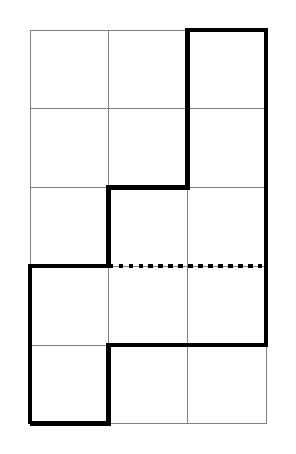
\begin{tikzpicture}
            \draw[help lines] (0,0) grid (3,5);
            \draw[ultra thick] (0,0) -- (1,0) -- (1,1) -- (3,1) -- (3,5) --
                         (2,5) -- (2,3) -- (1,3) -- (1,2) -- (0,2) -- (0,0);
            \draw[ultra thick,dotted] (1,2) -- (3,2);
            \end{tikzpicture}
        \end{center}
    }

    \example
    {
        6 \newline
        0 0 \newline
        1 0 \newline
        1 1 \newline
        2 1 \newline
        2 2 \newline
        0 2
    }
    {
        NO
    }
    {
        Hier gibt es keine Möglichkeit, das Köngigreich in zwei kongruente Teile zu teilen.
        \begin{center}
            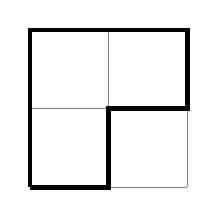
\begin{tikzpicture}
            \draw[help lines] (0,0) grid (2,2);
            \draw[ultra thick] (0,0) -- (1,0) -- (1,1) --
                         (2,1) -- (2,2) -- (0,2) -- (0,0);
            \end{tikzpicture}
        \end{center}
    }

    \Scoring

    \begin{description}
        \item[Teilaufgabe 1 (12 points).] $4 \le N \le 100\ 000$.
        Jede horizontale oder vertikale Gerade, die das Polygon zerteilt, zerteilt es in genau zwei Teile.        
        \item[Teilaufgabe 2 (15 points).] $4 \le N \le 200$.
        \item[Teilaufgabe 3 (23 points).] $4 \le N \le 4\ 000$.
        \item[Teilaufgabe 4 (50 points).] $4 \le N \le 100\ 000$.
    \end{description}

    \Constraints

    \begin{description}
        \item[Zeitlimit:] 0.5 s.
        \item[Speicherlimit:] 256 MB.
    \end{description}

\end{document}
